\Subsection{mvars}{Communication: MVars}

The lowest-level communication abstraction in Concurrent Haskell is
the @MVar@, whose interface is given below:

\begin{haskell}
data MVar a  -- abstract

newEmptyMVar :: IO (MVar a)
newMVar      :: a -> IO (MVar a)
takeMVar     :: MVar a -> IO a
putMVar      :: MVar a -> a -> IO ()
\end{haskell}

\noindent An @MVar@ can be thought of as a box that is either empty
or full. The @newEmptyMVar@ operation creates a new empty box, and @newMVar@ creates
a new full box containing the value passed as its argument.  The @putMVar@
operation puts a value into the box, but blocks (waits) if the box is
already full.  Symmetrically, the @takeMVar@ operation removes the value
from a full box but blocks if the box is empty.

@MVar@s generalise several simple concurrency abstractions:

\begin{itemize}
\item @MVar ()@ is a \emph{lock}; @takeMVar@ acquires the lock and
  @putMVar@ releases it again.\footnote{It works perfectly well the
    other way around too, just be sure to be consistent about the policy.}  An @MVar@ used in this way can protect
  shared mutable state or critical sections.

\item An @MVar@ is a one-place channel, which can be used for
  asynchronous communication between two threads.  In
  \secref{channels} we show how to build unbounded buffered channels
  from @MVar@s.

\item An @MVar@ is a useful container for shared mutable state.  For
  example, a common design pattern in Concurrent Haskell when several
  threads need read and write access to some state, is to represent
  the state value as an ordinary immutable Haskell data structure
  stored in an @MVar@.  Modifying the state consists of taking the
  current value with @takeMVar@ (which implicitly acquires a lock),
  and then placing a new value back in the @MVar@ with @putMVar@
  (which implicitly releases the lock again).

% ToDo:
% We'll come back to shared mutable state in \secref{conc-data}.
\end{itemize}

We can also use @MVar@s to do some simple asynchronous I/O.  Suppose
we want to download some web pages concurrently and wait for them all
to download before continuing.  We are given the following function to
download a web page:

\begin{haskell}
getURL :: String -> IO ByteString
\end{haskell}

\noindent Let's use this to download two URLs concurrently:

\begin{numhaskell}
do
   m1 <- newEmptyMVar
   m2 <- newEmptyMVar

   forkIO $ do
     r <- getURL "http://www.wikipedia.org/wiki/Shovel"
     putMVar m1 r

   forkIO $ do
     r <- getURL "http://www.wikipedia.org/wiki/Spade"
     putMVar m2 r

   r1 <- takeMVar m1
   r2 <- takeMVar m2
   return (r1,r2)
\end{numhaskell}

\noindent Lines 2--3 create two new empty @MVar@s to hold the
results.  Lines 5--7 fork a new thread to download the first URL; when
the download is complete the result is placed in the @MVar@ @m1@, and
lines 9--11 do the same for the second URL, placing the result in @m2@.
In the main thread, line 13 waits for the result from @m1@, and line 14
waits for the result from @m2@ (we could do these in either order), and
finally both results are returned.

This code is rather verbose.  We could shorten it by using various
existing higher-order combinators from the Haskell library, but a
better approach would be to extract the common pattern as a new
abstraction: we want a way to perform an action \emph{asynchronously},
and later wait for its result.  So let's define an interface that does
that, using @forkIO@ and @MVar@s:

\begin{numhaskell}
newtype Async a = Async (MVar a)

async :: IO a -> IO (Async a)
async io = do
  m <- newEmptyMVar
  forkIO $ do r <- io; putMVar m r
  return (Async m)

wait :: Async a -> IO a
wait (Async m) = readMVar m
\end{numhaskell}

\noindent Line 1 defines a datatype @Async@ that represents an
asynchronous action that has been started.  Its implementation is just
an @MVar@ that will contain the result; creating a new type here might
seem like overkill, but later on we will extend the @Async@ type to
support more operations, such as cancellation.

The @wait@ operation uses @readMVar@, defined
thus\footnote{@readMVar@ is a standard operation provided by
  the @Control.Concurrent@ module}:

\begin{haskell}
readMVar :: MVar a -> IO a
readMVar m = do
  a <- takeMVar m
  putMVar m a
  return a
\end{haskell}

\noindent that is, it puts back the value into the @MVar@ after
reading it, the point being that we might want to call @wait@ multiple
times, or from different threads.

Now, we can use the @Async@ interface to clean up our
web-page downloading example:

\begin{numhaskell}
do
   a1 <- async $ getURL "http://www.wikipedia.org/wiki/Shovel"
   a2 <- async $ getURL "http://www.wikipedia.org/wiki/Spade"
   r1 <- wait a1
   r2 <- wait a2
   return (r1,r2)
\end{numhaskell}

Much nicer!  To demonstrate this working, we can make a small wrapper
that downloads a URL and reports how much data was downloaded and how
long it took\footnote{the full code can be found in the sample @geturls.hs@}:

\begin{haskell}
sites = ["http://www.google.com",
         "http://www.bing.com",
         ... ]

main = mapM (async.http) sites >>= mapM wait
 where
   http url = do
     (page, time) <- timeit $ getURL url
     printf "downloaded: %s (%d bytes, %.2fs)\n"
        url (B.length page) time
\end{haskell}

\noindent which results in something like this:

{\scriptsize
\begin{verbatim}
downloaded: http://www.google.com (14524 bytes, 0.17s)
downloaded: http://www.bing.com (24740 bytes, 0.18s)
downloaded: http://www.wikipedia.com/wiki/Spade (62586 bytes, 0.60s)
downloaded: http://www.wikipedia.com/wiki/Shovel (68897 bytes, 0.60s)
downloaded: http://www.yahoo.com (153065 bytes, 1.11s)
\end{verbatim}
}

\begin{figure}
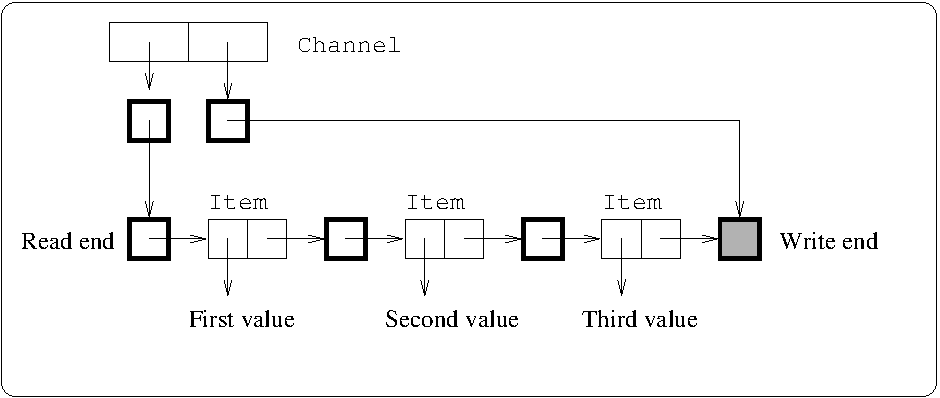
\includegraphics[scale=0.8]{channel.pdf}
\label{fig:channels}
\caption{Structure of the buffered channel implementation}
\end{figure}

\Subsubsection{channels}{Channels}

One of the strengths of @MVar@s is that they are a useful building
block out of which larger abstractions can be constructed.  Here we
will use @MVar@s to construct a unbounded buffered channel, supporting
the following basic interface:

\begin{haskell}
data Chan a

newChan   :: IO (Chan a)
readChan  :: Chan a -> IO a
writeChan :: Chan a -> a -> IO ()
\end{haskell}

\noindent This channel implementation first appeared in
\citet{jones96concurrent} (although the names were slightly
different), and is available in the Haskell module
@Control.Concurrent.Chan@.  The structure of the implementation is
represented diagrammatically in \figref{channels}, where each bold box
represents an @MVar@ and the lighter boxes are ordinary Haskell data
structures.  The current contents of the channel are represented as a
@Stream@, defined like this:

\begin{haskell}
type Stream a = MVar (Item a)
data Item a   = Item a (Stream a)
\end{haskell}

\noindent The end of the stream is represented by an empty @MVar@,
which we call the ``hole'', because it will be filled in when a new
element is added.  The channel itself is a pair of @MVar@s, one
pointing to the first element of the @Stream@ (the read position), and
the other pointing to the empty @MVar@ at the end (the write
position):

\begin{haskell}
data Chan a
 = Chan (MVar (Stream a))
        (MVar (Stream a))
\end{haskell}

To construct a new channel we must first create an empty @Stream@, which
is just a single empty @MVar@, and then the @Chan@ constructor with
@MVar@s for the read and write ends, both pointing to the empty
@Stream@:

\begin{haskell}
newChan :: IO (Chan a)
newChan = do
   hole  <- newEmptyMVar
   readVar  <- newMVar hole
   writeVar <- newMVar hole
   return (Chan readVar writeVar)
\end{haskell}

To add a new element to the channel we must make an @Item@ with a new
hole, fill in the current hole to point to the new item, and adjust
the write-end of the @Chan@ to point to the new hole:

\begin{haskell}
writeChan :: Chan a -> a -> IO ()
writeChan (Chan _ writeVar) val = do
  new_hole <- newEmptyMVar
  old_hole <- takeMVar writeVar
  putMVar writeVar new_hole
  putMVar old_hole (Item val new_hole)
\end{haskell}

To remove a value from the channel, we must follow the read end of the
@Chan@ to the first @MVar@ of the stream, take that @MVar@ to get the
@Item@, adjust the read end to point to the next @MVar@ in the stream,
and finally return the value stored in the @Item@:

\begin{numhaskell}
readChan :: Chan a -> IO a
readChan (Chan readVar _) = do
  stream <- takeMVar readVar
  Item val new <- takeMVar stream
  putMVar readVar new
  return val
\end{numhaskell}

\noindent Consider what happens if the channel is empty.  The first
@takeMVar@ (line 3) will succeed, but the second @takeMVar@ (line 4)
will find an empty hole, and so will block.  When another thread calls
@writeChan@, it will fill the hole, allowing the first thread to
complete its @takeMVar@, update the read end (line 5) and finally
return.

If multiple threads concurrently call @readChan@, the first one will
successfully call @takeMVar@ on the read end, but the subsequent
threads will all block at this point until the first thread completes
the operation and updates the read end.  If multiple threads call
@writeChan@, a similar thing happens: the write end of the @Chan@ is
the synchronisation point, only allowing one thread at a time to add
an item to the channel.  However, the read and write ends being
separate @MVar@s allows concurrent @readChan@ and @writeChan@
operations to proceed without interference.

This implementation allows a nice generalisation to \emph{multicast}
channels without changing the underlying structure.  The idea is to
add one more operation:

\begin{haskell}
dupChan :: Chan a -> IO (Chan a)
\end{haskell}

\noindent which creates a duplicate @Chan@ with the following
semantics:

\begin{itemize}
\item The new @Chan@ begins empty,
\item Subsequent writes to either @Chan@ are read from both; that is,
  reading an item from one @Chan@ does not remove it from the other.
\end{itemize}

The implementation is straightforward:

\begin{haskell}
dupChan :: Chan a -> IO (Chan a)
dupChan (Chan _ writeVar) = do
   hole       <- takeMVar writeVar
   putMVar writeVar hole
   newReadVar <- newMVar hole
   return (Chan newReadVar writeVar)
\end{haskell}

\noindent Both channels share a single write-end, but they have
independent read-ends.  The read end of the new channel is initialised
to point to the hole at the end of the current contents.

Sadly, this implementation of @dupChan@ does not work!  Can you see
the problem?  The definition of @dupChan@ itself is not at fault, but
combined with the definition of @readChan@ given earlier it does not
implement the required semantics.  The problem is that @readChan@ does
not replace the contents of a hole after having read it, so if
@readChan@ is called to read values from both the channel returned by
@dupChan@ and the original channel, the second call will block.  The fix is to change a
@takeMVar@ to @readMVar@ in the implementation of @readChan@:

\begin{numhaskell}
readChan :: Chan a -> IO a
readChan (Chan readVar _) = do
  stream <- takeMVar readVar
  Item val new <- readMVar stream -- modified
  putMVar readVar new
  return val
\end{numhaskell}

\noindent Line 4 returns the @Item@ back to the @Stream@, where it can
be read by any duplicate channels created by @dupChan@.

Before we leave the topic of channels, consider one more extension to
the interface that was described as an ``easy extension'' and left as
an exercise by \citet{jones96concurrent}:

\begin{haskell}
unGetChan :: Chan a -> a -> IO ()
\end{haskell}

\noindent the operation @unGetChan@ pushes a value back on the read
end of the channel.  Leaving aside for a moment the fact that the
interface does not allow the atomic combination of @readChan@ and
@unGetChan@ (which would appear to be an important use case), let us
consider how to implement @unGetChan@.  The straightforward
implementation is as follows:

\begin{numhaskell}
unGetChan :: Chan a -> a -> IO ()
unGetChan (Chan readVar _) val = do
   new_read_end <- newEmptyMVar
   read_end <- takeMVar readVar
   putMVar new_read_end (Item val read_end)
   putMVar readVar new_read_end
\end{numhaskell}

\noindent we create a new hole to place at the front of the @Stream@
(line 3), take the current read end (line 4) giving us the current
front of the stream, place a new @Item@ in the new hole (line 5), and
finally replace the read end with a pointer to our new item.

Simple testing will confirm that the implementation works.  However,
consider what happens when the channel is empty, there is already a
blocked @readChan@, and another thread calls @unGetChan@.  The desired
semantics is that @unGetChan@ succeeds, and @readChan@ should return
with the new element.  What actually happens in this case is deadlock:
the thread blocked in @readChan@ will be holding the read-end @MVar@,
and so @unGetChan@ will also block (line 4) trying to take the read
end.  As far as we know, there is no implementation of @unGetChan@
that has the desired semantics.

The lesson here is that programming larger structures with @MVar@ can
be much trickier than it appears.  As we shall see shortly, life gets
even more difficult when we consider exceptions.  Fortunately there is
a solution, that we will describe in \secref{stm}.

Despite the difficulties with scaling @MVar@s up to larger
abstractions, @MVar@s do have some nice properties, as we shall see in
the next section.

\Subsubsection{fairness}{Fairness}

Fairness is a well-studied and highly technical subject, which we do
not attempt to review here.  Nevertheless, we wish to highlight one
particularly important guarantee provided by @MVar@s with respect to
fairness:

\begin{quote}
No thread can be blocked indefinitely on an @MVar@ unless another
thread holds that @MVar@ indefinitely.
\end{quote}

In other words, if a thread $T$ is blocked in @takeMVar@, and there
are regular @putMVar@ operations on the same @MVar@, then it is
guaranteed that at some point thread $T$'s @takeMVar@ will return.  In
GHC this guarantee is implemented by keeping blocked threads in a FIFO
queue attached to the @MVar@, so eventually every thread in the queue
will get to complete its operation as long as there are other threads
performing regular @putMVar@ operations (an equivalent guarantee
applies to threads blocked in @putMVar@ when there are regular
@takeMVar@s).  Note that it is not enough to merely \emph{wake up} the
blocked thread, because another thread might run first and take
(respectively put) the @MVar@, causing the newly woken thread to go to
the back of the queue again, which would invalidate the fairness
guarantee.  The implementation must therefore atomically wake up the
blocked thread \emph{and} perform the blocked operation, which is
exactly what GHC does.

\paragraph{Fairness in practice}  Recall our example from \secref{forking}, where we had two threads,
one printing @A@s and the other printing @B@s, and the output was
often perfect alternation between the two: @ABABABABABABABAB@.  This
is an example of the fairness guarantee in practice.  The @stdout@
handle is represented by an @MVar@, so when both threads attempt to
call @takeMVar@ to operate on the handle, one of them wins and the
other becomes blocked.  When the winning thread completes its
operation and calls @putMVar@, the scheduler wakes up the blocked
thread \emph{and} completes its blocked @takeMVar@, so the original
winning thread will immediately block when it tries to re-acquire the
handle.  Hence this leads to perfect alternation between the two
threads.  The only way that the alternation pattern can be broken is if one
thread is pre-empted while it is not holding the @MVar@; indeed this
does happen from time to time, as we see the occasional long string of
a single letter in the output.

%  that this implementation does rely on some fairness in the
% scheduler too: the thread waiting to do the next @putMVar@ must not be
% indefinitely delayed, otherwise the fairness guarantee on @MVar@s
% fails.  At the current time GHC is using round-robin scheduling which
% satisfies this property.

A consequence of the fairness implementation is that, when multiple
threads are blocked, \emph{we only need to wake up a single thread}.
This single wakeup property is a particularly important performance
characteristic when a large number of threads are contending for a
single @MVar@.  As we shall see later, it is the fairness guarantee
together with the single-wakeup property which means that @MVar@s are
not completely subsumed by Software Transactional Memory.

